\documentclass[11pt,a4paper]{article}

\usepackage{color,graphicx,listings,wrapfig,hyperref,algpseudocode,mathtools}
\usepackage[margin=2cm,a4paper]{geometry}
\usepackage{algorithm}
\usepackage[toc,page]{appendix}

\graphicspath{{./img/}}

\begin{document}
\title{Message Passing Programming Project}
\author{c02f-32d66e}
\maketitle

\section{Introduction}
Our task in this assignment was to build an image-transforming parallel program using the \texttt{MPI library} for handling data transfer between processes.
The program applies an iterative method of recovering an original image from one containing a result of an edge detection algorithm. 
To enable more efficient use of resources, our program uses a 2D image decomposition to distribute parts of the image to appropriate processes. 
This ensures better performance and scaling characteristics than what would be available from a simple one-dimensional version, a discussion of which is presented in the later parts of the report.

This implementation of the problem solution does not try to make the code more advanced than what is required. 
Instead, we focused on ensuring we have created a complete, working and thoroughly tested code. 
We have put a lot of thought in the comments, code structure and documentation tools used, thus aiming to make the program easily understandable and modifiable by others. 
We firmly believe that great achievements come not only from individual brilliance, but from cooperation between people.

As we aimed for the code to resemble a real-life software project as closely as possible, the sources and all of their history is available as a \texttt{git} repository on \href{https://github.com/mkawalec/5thyear/tree/master/mpp/MPP-casestudy}{github}. 
The reader is encouraged to browse the code history to understand how certain ideas came to being and to posses a better grasp of the evolution of its structure to a present form.

\section{Pre-implementation considerations}
\subsection{Programming model}
\label{sec:model}
The three main ways in which the program could be structured we considered where: writing a monolithic code that would contain all the logic in a main function, branching out the most commonly used operations into separate functions or creating a self-contained library that could be used by the main function and would hide complexity inside the library itself.
The first option was excluded right away, as it quickly leads to creation of so called ``spaghetti code'' making understanding by others and subsequent code modifications exponentially harder as the development time progresses. 
By making the program hard to read it also encourages errors that are easy to avoid in a properly compartmentalised code and after a certain point it is impossible for the human brain to keep track of track dependencies between different program parts.

Both second and third way of structuring a \texttt{C} program have merit in various circumstances, and we decided to strike a balance between them. 
The most commonly used operations are branched into functions put in other source files, presenting an interface similar, but not identical, to respective functions provided by \texttt{MPI}.
The interface is kept program-specific, as we decided that complete versatility (as provided by \texttt{MPI}) is neither needed nor desirable in this project. 
By keeping interaction with functions specific to a problem at hand, we created a clear and concise code.
We also wrote the code in a way that would make it easy to apply our solution to a similar problem, at the same time making it quite simple to modify to enable, for instance, working on different data types.

Thus the structure we arrived at comprises of a \texttt{main} function performing operations the exact implementation of which is left for external functions to define. 
In addition to advantages mentioned above, such an approach makes it easy to reason about the code on the higher level encapsulating the complexity in layers of abstraction.

\subsection{Build system and documentation}
We have decided to use a widely tested and versatile build system and as such an obvious choice was the \texttt{GNU Make}. 
It would definitely suffice in the most simple of use cases, but it has several drawbacks. 
Most notably, it would require additional configuration to build an \texttt{MPI} program on some platforms. 
We wanted a tool more versatile and providing clearer syntax.
As such we chose \texttt{cmake}. 
It enables seamless use of various \texttt{MPI} implementations through the supplied find scripts. 
As it is also very easy to run documentation generating programs with, it was a good first choice.

For documentation generation, we used \texttt{Doxygen}. 
It is a de facto standard for \texttt{C}/\texttt{C++} documentation creation and generation. 
It is also easy to use and files documented in \texttt{Doxygen}-compatible way can easily be read raw or a generated documentation in any format can be viewed for added clarity and features.

\subsection{Testing}
After considering various options, we have decided not to use a unit-testing framework. 
This has certain drawbacks, but we assumed that given a small project size and simple operations applied, the vast majority of errors will originate from the interprocess communication and decomposition algorithms. 
We discovered during implementation phase that we were not mistaken. 

However, the source of errors is not in itself an argument against writing unit tests -- we could, after all, implement tests that check the correctness of decomposition algorithms.
We chose not to, as considerable time and effort would be exerted implementing tests that would only be practically needed if the program had prospects of further development and future growth, which it does not.

\section{Implementation}
\subsection{Style}
While writing the program we followed the \href{https://www.kernel.org/doc/Documentation/CodingStyle}{Kernel coding guidelines} when it comes to formatting the code, with a few modifications. 
We felt that 80 characters in a line is a better limit on line width and that indenting by four spaces is more readable than an eight-space option suggested by the guide. 

We preferred to put functionally related code in the same file and to keep the length of each file under five hundred lines if possible, to help readability and collaboration. 
The limit on file length was never reached as it is a relatively small project, but it is always good to be kept in mind when writing code.
In the end the codebase had evolved to span five source files and four headers with functions in different files having distinctly different applications.

\subsection{Data structures used}
There are three main data structures in use in the program and we will examine them one by one.
Exploration of usage scenarios for the following structures can be found in subsequent sections, most notably in~\ref{sec:2dscatgat}.

\subsubsection{Master buffer}
It is a simple array of floats to which the input file is read and the output is written from. 
The scatter and gather operations also use the master buffer as a source or a target, respectively. 
It contains enough elements to convey information about every pixel of the input image and no more. 
There are no halos allocated in the master buffer as they are not of its concern. 
The master buffer is only allocated on the master thread (the one with id 0), which enables the program to run on machines without enough memory to contain whole input image (with exception of the machine running process zero, of course).

\subsubsection{Process-local data buffer and 2D arrays}
A buffer called \texttt{buf} in the program code is used as an intermediate structure to which the data is sent by the scatter function and taken from by gather. 
It is a 1D array of floats that contains the same amount of elements as the number of pixels in the image part sent to a given process. 

Three 2D arrays, \texttt{edge}, \texttt{new} and \texttt{old} contain intermediate computation state and the halos. 
A halo is a border one pixel wide on edges of the image data that is swapped with adjacent processes every iteration.
The inner elements of the arrays are updated by the transformation loop every iteration.

\subsection{2D decomposition algorithm}
\label{sec:2ddec}
Choosing one algorithm over another is always a trade-off between implementation complexity, performance and correctness. We have decided to use a simple to implement algorithm that chooses the most efficient decomposition for most cases and when it does not it indicates that. The pseudo-code version of the decomposition algorithm is presented as Algorithm~\ref{2dcomp}.

\begin{algorithm}
    \caption{2D decomposition algorithm}\label{2dcomp}
    \begin{algorithmic}[1]
        \State $commsize\gets$ communicator size
        \State $circ\gets$ \texttt{MAX\_INT}
        \State $result\gets$ \texttt{NULL}

        \For{$1 \leq i \leq \sqrt(commsize)$}
            \If{$commsize \bmod i = 0$ \textbf{and} $circumference(i) < circ$}
                \State $circ\gets circumference(i)$
                \State $result\gets i$
            \EndIf
        \EndFor
    \end{algorithmic}
\end{algorithm}

After the algorithm completes, $result$ will contain the number of chunks in the Y direction of the most efficient decomposition. 
The number of elements in the X dimension is trivially computed as $ceil(commsize / result)$. 
This algorithm uses a $circumference(i)$ method that returns a total circumference for a given number of divisions in Y direction. 
The total circumference is a measure that is proportional\footnote{Total circumference as defined in this implementation is proportional but slightly higher than the total amount of data exchanged in a simulation step as it also includes the ``corners'' of a halo, which are not sent.} to a complete amount of data that needs to be exchanged in one simulation step and needs to be minimised for a most efficient decomposition. 

In case the number of chunks in any direction does not divide the number of pixels in that direction evenly, the chunks most to the right (in case of X unevenness) or to the bottom will be smaller. 
It is a reasonable trade-off to make, as in all but the most malformed cases the difference in size between those side chunks and the inner ones will be minimal. 
In exchange we get a straightforward algorithm producing the chunks.

The algorithm, or rather the way it is used in this code, has one issue that is not immediately obvious and produces serious consequences at certain times. 
If we try to divide an image of a size 768 by 1152 pixels into 59 chunks, the algorithm says we should have 59 elements in Y direction and one in X as 59 is a prime number. 
We then proceed to divide 1152 by 59 to get the height of a chunk in pixels and we get $\approx 19.53$. 
This leaves us with two choices -- either have the chunks 19 or 20 pixels high. But if we choose 19, $1152 / 19\approx 60$ and if 20, $1152 / 20\approx 58$! So in neither of the two cases we get the correct number of chunks.

This issue can of course be solved if we give the program the freedom to make the last chunk row or column much bigger (or smaller) than the inner chunks, but such functionality was not implemented as it would increase code complexity and lead to poorer performance. 
Additionally, it only comes into play for certain uncommon numbers of created processes, and if such a situation occurs the program can notice it and refuse to continue.

\subsection{2D scatter/gather}
\label{sec:2dscatgat}
We decided to implement our 2D scatter and gather routines such that they would be callable in a similar way to the original \texttt{MPI} methods. 
The different behaviour for different ranks is hidden inside the body of the scatter and gather functions so that their user (be that another person or just the \texttt{main} function) calls them the same way from all the processes. 
We have omitted both the file type specification and indication of which process has the data to be scattered from the function call, as we feel that this loss of generality pays back with increased simplicity. 

A case could be made that this makes those functions that are quite general in nature very problem-specific, but we do not think that is an issue. 
If a greater generality would be needed (for instance for a 2D decomposition of a different data type or from a different process) a simple change can be made that would enable either of these functions to accept different data types or sources. 
But since these functions will only be used in this specific problem and no extensions are planned to the codebase, omitting these arguments only brings advantages from simplicity.

\subsubsection{Scatter algorithm analysis}
The scatter algorithm pseudocode is presented as Algorithm~\ref{2dscat}. 
First, an optimal decomposition is determined (line 1). 
Then, if the current process is a sending process, appropriate regions of the send buffer are sent to correct processes (lines 5 -- 11) in a non-blocking way. 
Then the data is received by a target process to a receive buffer and inverted. In the end, the receiving process waits until all the sending operations finish before finishing the function (lines 15 -- 16).

Two issues warrant increased attention here. 
First of all, the \texttt{invert} function inverts the contents of the buffer vertically. 
It is needed, as the 2D topology generated by \texttt{MPI} uses process indexing which is the same as \texttt{C} array indexing with inverted Y axis. 
Without the invert operation on line 14 the user would need to send the upper halo to the bottom neighbour and the bottom halo to upper neighbour. 
We assumed that it would be better to shield the user of this function from this inconvenience and simply invert the data inside the scatter algorithm itself. 

Secondly, the usage if \texttt{MPI\_Issend} instead of other send methods requires explanation. 
The usage of Bsend in this place would not bring any benefits to the program, as the buffer that needs to be allocated would need to be the size of the data being sent. 
That is not acceptable, as the program may deal with very large input data and there may not be enough memory available for allocation. 
Additionally, we do not want the master process to complete before all the requests have completed. 
Because of both of this disadvantages and no advantages, we have decided to use \texttt{MPI\_Issend}.

We have not chosen ``Standard send'' as we want to have more control over over how the data is sent than what this function allows. 
The ``Ready send'' mode was not even briefly considered, as it would provide ephemeral gains in this scenario while making is much harder to write a correct program.
\begin{algorithm}
    \caption{2D scatter algorithm}\label{2dscat}
    \begin{algorithmic}[1]
        \State $optimal\gets$ \texttt{decomposition\_length()}
        \State $rank\gets$ current rank
        \State $commsize\gets$ communicator size
        \State $send\_buf\gets$ send buffer

        \If{$rank = 0$}
        \State $dims\gets$ \texttt{decomposition\_size()}
            \For{$0 \leq i \leq commsize$}
                \State $exchage\_type\gets$ \texttt{create\_dtype}($i$, $dims$)
                \State \texttt{MPI\_Issend}($i$, $exchange\_type$, $send\_buf$)
            \EndFor
        \EndIf

        \State $receive\_buf\gets$ receive buffer
        \State \texttt{MPI\_Recv}($receive\_buf$, $0$)
        \State \texttt{invert}($receive\_buf$)

        \If{$rank = 0$}
            wait until all the send requests complete
        \EndIf
    \end{algorithmic}
\end{algorithm}

\subsubsection{Gather algorithm analysis}
The Gather algorithm is very similar in principle to the scatter algorithm provided above and thus we feel that providing it here in form of pseudo-code would be redundant -- interested readers should see the source code. 
The main conceptual difference between gather and scatter is the direction of data transfer. 
The small parts of the data are inverted and sent by all the processes to the 0th process. 
Then they are assembled in correct places in the master buffer and the gather is complete.

We do not use non-blocking receive routines as we feel that a slight speed boost achieved by them is easily offset by simpler and less bug-prone gather code. 
This is especially true as Gather is ran only once per program execution. 
Moreover the \texttt{VAMPIR} parallel trace tool reveals that adding blocking receives adds minimal overhead to the program execution, as the final gather operation takes less than 15ms with 16 threads.

\subsection{Main program loop}
After distributing the data across processes the main program loop is reached. It is composed of two parts, which we will discuss separately.

\paragraph{Communicating state}
Every certain number of iterations the program prints some information about its current state. 
It tells the user what the current iteration is and the average pixel value at this iteration.
Because the 0th thread is the one printing the information\footnote{It is guaranteed to exist, so it is a safe and simple choice of a printing thread. Additionally it has the most work to do, as it has to scatter and gather image data and would usually be the last thread to reach a certain stage.} the information about the average pixel value is reduced to it. 
In order to minimise rounding errors and the need for the 0th thread to know dimensions of image part each thread works on, the \texttt{MPI\_Reduce} operation sums values of every pixel in the image.
This way the average value is the total sum divided by the number of pixels in an image, which can easily be computed without any knowledge of decomposition topology.

Our program must also run for a certain number of iterations and finish when image changes every iteration by a value lower than a certain threshold.
In order to perform this operation all processes must agree on when an appropriate stopping moment happens.
To achieve this we use \texttt{MPI\_Allreduce} for computing a global maximum change between iterations coupled with a check by every process comparing the computed value to the threshold.
If the computed change is smaller than the threshold, each of the processes finishes its main loop.

\paragraph{Communication and image transformation}
We use an immediately returning Standard Send for sending halo data that needs to be exchanged every iteration with adjacent processes.
We then receive the data into appropriate halos of a current process and apply the transformation. 
Only after doing that we require the send requests to complete using \texttt{MPI\_Wait}, which prevents deadlock and effectively exploits the asynchronous nature of send requests we are using.
It also increases performance, as transformation can be applied to the image before the send requests complete.
As much as we would like to delay synchronisation of send requests even further it is not possible while keeping an answer correct, as the state of an array from which data is sent changes dramatically.
We swap an \texttt{old} array, which holds the previous iteration state with the \texttt{new} array holding the current state.
As this operation changes the place in memory to which \texttt{old} points, integrity of the send operation couldn't be ensured if \texttt{MPI\_Wait} was delayed even further.

To ensure clear definitions of ``upper'' and ``lower'' halos we employ a virtual datatype anchored at a different place in the array.
Our partitioning scheme ensures that upper and lower neighbours of a process (determined with a help from \texttt{MPI} virtual topologies) have appropriate halos of the same size as the current process.

\subsection{Ensuring correctness}
\label{sec:correctness}
The question of a correct result in a parallel setting is an inherently complex one. 
How would one ensure a correct result when unpredictable events during communication can happen and when timing of operations is not guaranteed?
We have eliminated a possibility of a deadlock arising from the way communication is structured completely, by using a combination of asynchronous sends and synchronous receives placed in a correct order.
However, a deadlock arising from a hardware error of some sort is still possible and increases its probability as the program is scaled to more and more processors.
It it very possible to protect against such an error in software, but it is way beyond the scope of the current assignment and thus this avenue is left unexplored.

\paragraph{Data hashing}
Even though a deadlock is not possible, it still doesn't guarantee correctness of an answer.
For that we employed a two-part scheme.
After every run a probabilistic image hash is generated.
Its value is then compared to a known hash value of a result which correctness can be inspected visually.

The hash function we chose selects a certain number of pixels from the image at random, multiplies the values at the pixels by random numbers and outputs the result.
Because a certain preselected seed is set at the beginning of the function run we have a guarantee that for the same image the hash value will be the same.
Additional advantage of this scheme is that hashes of two similar images are similar.
We thought that such property would be needed as we deal with floating point numbers and certain small errors would be inevitable.
As it turned out no errors were observed.

The reason why we choose the pixels creating the hash at random are not due to performance in this setting.
We do it simply because \texttt{unsigned long long} is used for the hash value.
\texttt{GCC} implementation of RNG uses a range from $0$ to $10^9$ for the generated numbers, so using all the pixels would cause an overflow in cache value.
This also means that using the program with images that have more than 100 megapixels would cause a cache value overflow.
This problem could be solved by using a library supporting unlimited precision numbers for expressing the cache value, or implementing this simple functionality ourselves.
Again, such a functionality is outside of the scope of this project and was not realised in current code version.


\section{Results}
The results are presented here with lines depicting scaling properties of different input image sizes.
Of course it is impossible to run a program on a non-integer number of processors so all the following plots must be interpreted with this in mind.
Additionally, there are certain numbers of processors for which a decomposition is impossible using an algorithm described above.
Such cases are omitted from the plots.
Therefore, even if a straight line passes though a certain number of processors it does not mean that it is possible to run the program on this number of processors.
Only where a vertex is visible on a line an actual data point was recorded.

We were unsure if running the program just once would provide sufficiently accurate results.
To check that the program was ran multiple times for test data and differences in time between different runs were lower than 1\%.
Because of that, we have decided to execute each run case just once and take its value -- no additional statistical insight can be gained from running the program more times.

\subsection{Scaling properties}
\subsubsection{Big images}
The program exhibits expected behaviour when it comes to the execution time on increasing number of processors.
As can be observed on Figure~\ref{fig:big}, the execution time decreases with increasing numbers of processors until it stabilizes at a certain value, which cannot be lowered with an increase in the number of processes.
There are certain processor numbers for which the time is markedly higher then for neighbouring points.
It happens because it is impossible to decompose the image into a given number of parts effectively thus creating a 1D decomposition yielding inadequate performance.

\begin{figure}[h!]
    \begin{center}
        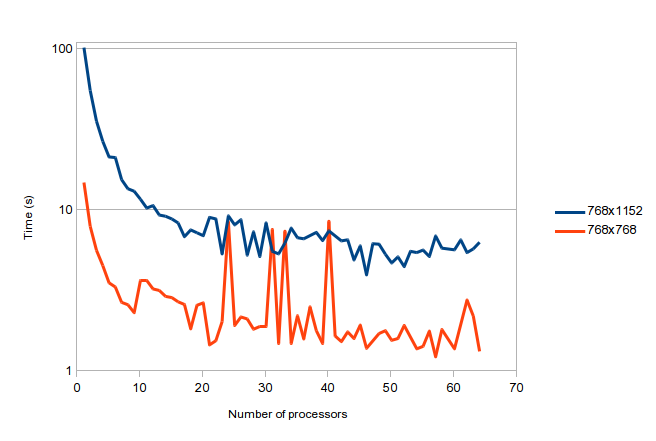
\includegraphics[width=0.8\textwidth]{big_time.png}
    \end{center}
    \caption{Execution times for two of the biggest images provided with the project. Notice that the time scale is logarithmic.}\label{fig:big}
\end{figure}

It is interesting to look at the big difference in execution times between these two images of similar sizes.
The bigger image contains only 50\% more pixels that the smaller one, yet the time difference between the two is of an order of 700\% in the worst case!
While \texttt{VAMPIR} helps with determining the reasons for the difference in times at higher number of processors (more time is spent communicating halos, the time needed for that increases faster than linearly), we were unable to understand the sources of the time difference at low processor counts.
We expected the difference to stem from a different time of the initial scatter and gather, but both are finished in a time of order of milliseconds and cannot be an issue here.
Additional investigation will need to be performed in order to resolve this issue.

\subsubsection{Small images}
\begin{wrapfigure}{r}{0.5\textwidth}
    \vspace{-60pt}
    \begin{center}
        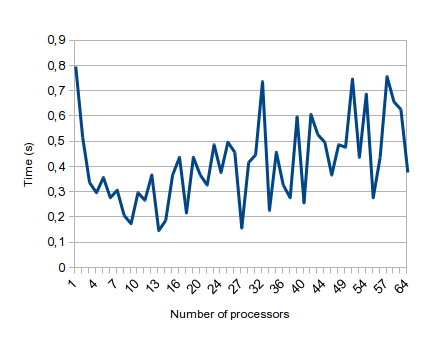
\includegraphics[width=0.48\textwidth]{small_time.png}
    \end{center}
    \vspace{-30pt}
    \caption{Execution time for the smallest image, with domination by communication costs at higher processor counts easily visible.}\label{fig:small}
    \vspace{-30pt}
\end{wrapfigure}

The small image execution time at higher number of processors (presented at Figure~\ref{fig:small}) is dominated by communication time.
It is also harder do create an efficient decomposition as the number of pixels in the image is small, explaining huge variations execution time between similar number of processors.
Also, as most of the time is spent communicating due to a limited amount of data being worked on, the effect of inefficient decompositions is more marked than in the case of the bigger images described above.
These predictions were confirmed by \texttt{VAMPIR} trace tool.

\subsubsection{Discussion of scaling effectiveness}
Presenting the above results on a speedup plot shows clearly how performance depends on the number of processors.
Figure~\ref{fig:speedup} clearly presents the relatively poor performance on the small input image and provides new insights into the behaviour with the biggest amount of data.
Interpreting it we can recommend that the program should be ran with the biggest dataset on 17 processors for an optimal performance.

This is a surprising result in itself. 
17 is a prime number, and as such it forces a one-dimensional decomposition to be applied to the image.
We did not expect the gains achieved from less send operations to outweigh the benefits from less data transferred in each request at this image size.
Given that we suggest that the program should be ran with much bigger datasets to achieve the full potential of the 2D decomposition.

\begin{figure}[h!]
    \begin{center}
        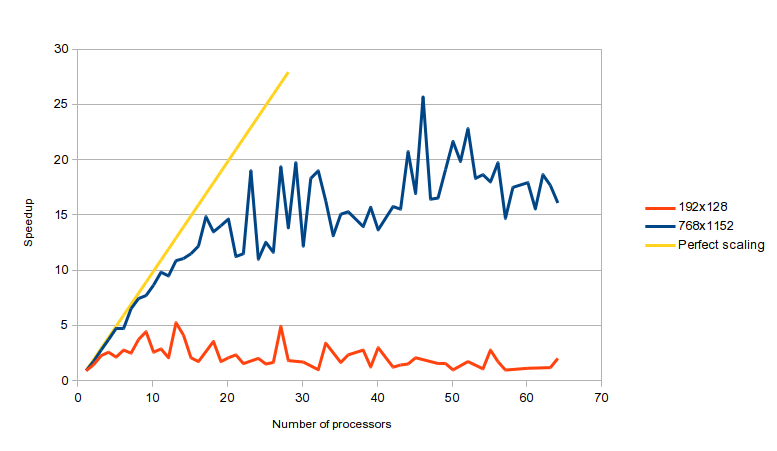
\includegraphics[width=0.8\textwidth]{speedup.png}
    \end{center}
    \caption{Comparison of parallel speedup for different processor numbers and image sizes. A part of perfect scaling line is provided as reference}\label{fig:speedup}
\end{figure}

We have omitted the results from other image sizes than the most extreme ones from this plot to enhance clarity and provide a clear view to the reader.

\subsection{Correctness checking}
\paragraph{Image correctness}
The hashing scheme described in Section~\ref{sec:correctness} performed well, giving different results for different images, as expected.
It had also assured us that results obtained from different runs had produced the same, correct image as the one verified visually for the serial solution.

\paragraph{Program correctness}
Even though the results provided by the program were correct and exhibited expected scaling properties, we performed additional checks to ensure that there were no errors made during implementation.
We have checked the program with \texttt{memcheck} tool from \texttt{valgrind} suite.
It had indicated that no memory leaks occur in our code, even though there could be memory leaks related to the way \texttt{MPI} handles parallel connections.
Running the program through a profiler included with \texttt{valgrind}, \texttt{callgrind} indicated little time spend on communication and overall the expected performance profile.

\subsection{Issues with compilation on cplab machines}
We have experienced some issues related to \texttt{cmake} when compiling our code on \texttt{cplab} machines with \texttt{MPICH2}.
For simplicity, and since the problems encountered are due to an old \texttt{MPICH2} version on the aforementioned machines, we have provided a pre-compiled executable that runs successfully in this environment.
For more information, please see Appendinx~\ref{sec:comp}.

\section{Conclusion}
An implementation of a two-dimensional parallel image recovery program was presented.
Its correctness was checked and ensured through multiple layers of checks and up to the best of our knowledge a correct result was produced for every run case.
We have observed an expected scaling behaviour in parallel execution which confirmed the efficiency of our implementation.

Certain avenues of possible future improvement were also proposed and their merit discussed.
We have implemented none of them as we felt our effort would be much better spent on producing a clear, concise and well documented code.
Trusting that we have managed to do exactly that we present the code to you and wait anxiously for your opinion on this subject.
A quick start guide is included at the end of this report to help the reader compile and run the program by herself.



\newpage
\begin{appendices}
\section{Quick start guide}
\subsection{Compiling the program}
\label{sec:comp}
In order to compile the program the following sequence of commands needs to be executed.

\vspace{5pt}
\noindent \texttt{mkdir build}

\noindent \texttt{cd build \&\& cmake ..}

\noindent \texttt{make}
\vspace{5pt}

\noindent As mentioned earlier, when running on \texttt{cplab} machines you are advised to skip the compilation steps and simply run an executable from \texttt{data} directory.
Keep in mind that apart from the expected \texttt{MPI} dependencies, the program requires OpenMP (used here for time measurement).

\noindent To build documentation (provided \texttt{Doxygen} is available on your system) execute the following from inside the \texttt{build} directory:

\vspace{5pt}
\noindent \texttt{make doc}
\vspace{5pt}

\subsection{Running the program}
The program accepts command line arguments in a following format:

\vspace{5pt}
\noindent \texttt{./edges input\_image x\_dimension y\_dimension}
\vspace{5pt}

\noindent That means that running the program with the biggest image as input has the form:

\vspace{5pt}
\noindent \texttt{./edges data/edge768x1152.pgm 768 1152}
\vspace{5pt}

\noindent The above pattern can be adapted to any input image in PGM format.

\end{appendices}

\end{document}
